\section{预条件}
\label{sec:ls-preconditioning}

前面各节的求解器规定了在Krylov子空间中怎样选解，但要多少步才能达到所需精度，取决于系数矩阵本身。本节讨论一种不改变求解器、只改变它所面对的矩阵的加速手段，即预条件。下面先说明为什么需要它、它的基本做法，再介绍三种常用的预条件矩阵，最后说明怎样把预条件放进具体的求解器中。

\subsection{主要思想}

Krylov方法的收敛快慢由系数矩阵的谱决定。以CG为例，定理~\ref{thm:ls-cg-convergence}给出的误差界每步乘以因子
\[
 \frac{\sqrt\kappa-1}{\sqrt\kappa+1},\qquad \kappa=\kappa_2(\bm A).
\]
条件数$\kappa$越大，这个因子越接近$1$，误差下降越慢，达到同一精度所需的步数大致与$\sqrt\kappa$成正比。其他方法虽然没有这样简单的界，但道理相同：特征值或奇异值分布得越开，要压低残差所需的多项式次数就越高，步数也越多。

实际问题中的矩阵常常条件很差。偏微分方程离散化时，网格越细，条件数增长越快；各个未知量的单位或量级相差悬殊时，特征值也会分布得很开。这时Krylov方法要走很多步，每一步的矩阵乘向量与正交化都要付出代价。预条件的想法是：既然步数由矩阵决定，就先把方程改写成一个同解、但矩阵条件更好的方程，再交给求解器。

\term{预条件}（preconditioning）选一个可逆矩阵$\bm M$，它满足两个要求：一是在某种意义上接近$\bm A$；二是以$\bm M$为系数的方程$\bm M\bm z=\bm r$容易求解。把$\bm A\bm x=\bm b$两边左乘$\bm M^{-1}$，得到同解方程
\[
 \bm M^{-1}\bm A\bm x=\bm M^{-1}\bm b .
\]
求解器面对的矩阵就从$\bm A$变成了$\bm M^{-1}\bm A$。$\bm M$越接近$\bm A$，$\bm M^{-1}\bm A$越接近单位矩阵，它的特征值就越集中在$1$附近，条件数越小，所需的步数也越少。

两个要求是相互牵制的。取$\bm M=\bm A$时，$\bm M^{-1}\bm A=\bm I$，一步就能结束，但解$\bm M\bm z=\bm r$与解原方程一样难；取$\bm M=\bm I$时，辅助方程无须求解，但矩阵也没有任何改善。实用的预条件介于两者之间：每步多付出一次廉价的辅助求解，换来步数的明显减少。

实现时既不求$\bm M^{-1}$，也不形成$\bm M^{-1}\bm A$。求解器每次需要$\bm M^{-1}$作用在某个向量$\bm r$上时，就解一次辅助方程$\bm M\bm z=\bm r$，取其解$\bm z$。这一次求解的代价最好与一次矩阵乘向量相当。另外，$\bm M$在整个求解过程中必须固定不变。若$\bm M$逐步改变，求解器面对的矩阵也随之改变，前面各节证明的正交性与最优性就都不再成立。

于是，使用预条件要回答两个问题：怎样构造这样的$\bm M$，以及在求解器中怎样使用它。下面两小节依次回答。

\subsection{常见预条件方法}
\label{sec:ls-preconditioner-constructions}

构造$\bm M$不需要新的工具，前面几章的方法就够用。对角预条件与SSOR预条件取自第~\ref{chap:stationary-iterations}章定常迭代的分裂，不完全分解取自第~\ref{chap:direct-linear-solvers}章的LU与Cholesky分解。三者由简到繁：越复杂的$\bm M$越接近$\bm A$，效果越好，构造与求解的代价也越高。下面都用例~\ref{ex:ls-stationary-running-example}的矩阵演示，看所得的$\bm M$与$\bm A$差在哪里：
\[
 \bm A=\begin{bmatrix}4&1\\1&3\end{bmatrix}.
\]

\subsubsection{对角预条件}
\label{sec:ls-diagonal-preconditioning}

\paragraph{构造}
最简单的近似是只保留$\bm A$的对角部分：
\begin{equation}
 \bm M=\operatorname{diag}(a_{1,1},\ldots,a_{d,d}),
 \label{eq:ls-diagonal-preconditioner-matrix}
\end{equation}
这就是第~\ref{sec:ls-jacobi}节Jacobi迭代所用的分裂矩阵，要求对角元都不为零。构造不需要任何计算。由于$\bm M$是对角矩阵，解$\bm M\bm z=\bm r$就是逐个分量相除：
\begin{equation}
 z_i=\frac{r_i}{a_{i,i}}\qquad(i=1,\ldots,d).
 \label{eq:ls-diagonal-preconditioner}
\end{equation}
例中
\[
 \bm M=\begin{bmatrix}4&0\\0&3\end{bmatrix},\qquad
 \bm M^{-1}\bm A=\begin{bmatrix}1&1/4\\1/3&1\end{bmatrix},
\]
$\bm M$与$\bm A$只差两个非对角元，$\bm M^{-1}\bm A$的对角元都变成了$1$。

\paragraph{性质}
左乘$\bm M^{-1}$相当于把第$i$个方程除以$a_{i,i}$，使各方程的对角元都变为$1$。所以对角预条件能消除各方程之间的尺度差异，但对非对角部分无能为力。$\bm A$对称正定时，它的对角元都为正，$\bm M$也对称正定。它不占额外存储，每次求解只需$d$次除法，是代价最小的预条件。

\paragraph{应用场景}
当各个方程或未知量的尺度相差很大，而病态主要由尺度造成时，对角预条件就很有效；它也常作为其他预条件之前的第一步。

下面的例子说明它的作用。取$d=10$，$\bm A=\bm S\bm T\bm S$，其中$\bm S=\operatorname{diag}(1,2,\ldots,10)$，$\bm T$是对角元为$1$、次对角元为$0.4$的三对角矩阵。$\bm T$本身条件很好，但两侧的$\bm S$使$\bm A$各行各列的尺度相差上百倍。

$\bm A$的对角部分恰为$\bm S^2$，取$\bm M=\bm S^2$，则
\[
 \bm M^{-1}\bm A=\bm S^{-1}\bm T\bm S ,
\]
它与$\bm T$相似，特征值为$1+0.8\cos(j\pi/11)$，$j=1,\ldots,10$。

图~\ref{fig:ls-preconditioned-spectrum}比较了两组特征值：$\bm A$的特征值从约$0.73$分布到约$133$，最大与最小之比约为$182.7$；缩放后全部落在$[0.23,1.77]$内，比值约为$7.61$。代入CG的误差界，每步的收缩因子从约$0.862$降到约$0.468$，而代价只是每步多做$d$次除法。

对最小二乘问题，同样的想法作用于列。记$\bm a_j$是$\bm A$的第$j$列，取
\[
 \bm M=\operatorname{diag}(\lVert\bm a_1\rVert_2,\ldots,\lVert\bm a_d\rVert_2),
\]
于是$\bm A\bm M^{-1}$的各列都是单位长度。这相当于对$\bm A^\top\bm A$作对角预条件。

\begin{figure}[htbp]
  \centering
  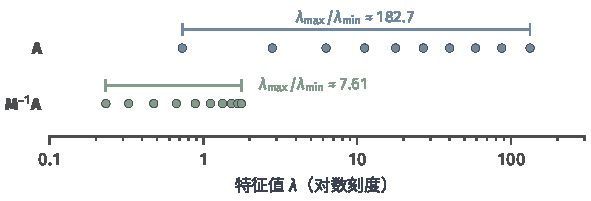
\includegraphics[width=100mm]{figures/01-basic-mathematics/03-vectors-matrices-and-multivariate-functions/matplotlib/c5-preconditioned-spectrum/figure.pdf}
  \caption{对角缩放前后的特征值分布（对数横轴）。矩阵为$\bm A=\bm S\bm T\bm S$，$\bm S=\operatorname{diag}(1,\ldots,10)$，$\bm T$为对角元$1$、次对角元$0.4$的三对角矩阵，预条件$\bm M=\operatorname{diag}(\bm A)$。蓝点为$\bm A$的$10$个特征值（数值计算），绿点为$\bm M^{-1}\bm A$的特征值$1+0.8\cos(j\pi/11)$；括线标出各自的范围与最大、最小特征值之比。}
  \label{fig:ls-preconditioned-spectrum}
\end{figure}

\subsubsection{SSOR预条件}

\paragraph{构造}
对角预条件丢掉了$\bm A$的全部非对角元。要保留更多信息，可以借用第~\ref{sec:ls-ssor}节的SSOR迭代。把对称矩阵写成
\[
 \bm A=\bm D+\bm L+\bm L^\top ,
\]
其中$\bm D$是对角部分，$\bm L$是严格下三角部分。SSOR迭代每一轮先作一次前向扫掠、再作一次反向扫掠，把残差$\bm r_k$变成修正量$\bm\delta_k$（式~\eqref{eq:ls-ssor-correction}）。这一修正是$\bm r_k$的线性函数，记作$\bm\delta_k=\bm M^{-1}\bm r_k$，其中
\begin{equation}
 \bm M=\frac{1}{\omega(2-\omega)}(\bm D+\omega\bm L)\bm D^{-1}(\bm D+\omega\bm L)^\top,\qquad 0<\omega<2 .
 \label{eq:ls-ssor-preconditioner-matrix}
\end{equation}
这个$\bm M$就是SSOR预条件。取$\omega=1$时展开可得
\begin{equation}
 \bm M=(\bm D+\bm L)\bm D^{-1}(\bm D+\bm L^\top)=\bm A+\bm L\bm D^{-1}\bm L^\top ,
 \label{eq:ls-ssor-preconditioner-difference}
\end{equation}
即$\bm M$与$\bm A$只差一项$\bm L\bm D^{-1}\bm L^\top$。

求解$\bm M\bm z=\bm r$不需要形成$\bm M$。记$\bm F=\bm D+\omega\bm L$，它是下三角矩阵，于是$\bm M\bm z=\bm r$可以拆成三步：先解下三角方程，再作对角缩放，最后解上三角方程，
\begin{equation}
 \bm F\bm y=\bm r,\qquad \bm t=\omega(2-\omega)\bm D\bm y,\qquad \bm F^\top\bm z=\bm t .
 \label{eq:ls-ssor-preconditioner}
\end{equation}
三步依次给出$\bm y=\bm F^{-1}\bm r$与$\bm z=\bm F^{-\top}\bm t$，合起来正是
\[
 \bm z=\omega(2-\omega)\bm F^{-\top}\bm D\bm F^{-1}\bm r=\bm M^{-1}\bm r .
\]

例中取$\omega=1$，严格下三角部分与修正项为
\[
 \bm L=\begin{bmatrix}0&0\\1&0\end{bmatrix},\qquad
 \bm L\bm D^{-1}\bm L^\top=\begin{bmatrix}0&0\\0&1/4\end{bmatrix},
\]
所以
\[
 \bm M=\begin{bmatrix}4&1\\1&13/4\end{bmatrix},
\]
它与$\bm A$只在右下角差$1/4$，比对角预条件接近得多。

对$\bm r=(1,2)^\top$求解一次。前代、缩放与回代依次得到
\[
 \bm y=\begin{bmatrix}1/4\\7/12\end{bmatrix},\qquad
 \bm t=\bm D\bm y=\begin{bmatrix}1\\7/4\end{bmatrix},\qquad
 \bm z=\begin{bmatrix}5/48\\7/12\end{bmatrix}.
\]
这正是第~\ref{sec:ls-ssor}节从零初值作一轮SSOR迭代得到的$\bm x_1$。

\paragraph{性质}
SSOR预条件保留了$\bm A$的全部元素，只多出一项$\bm L\bm D^{-1}\bm L^\top$（$\omega=1$时），通常比对角预条件更接近$\bm A$。$\bm A$对称正定且$0<\omega<2$时，$\bm M$也对称正定。它不需要额外存储：所用的三角矩阵$\bm F$就是$\bm A$的下三角部分。每次求解相当于两次三角扫掠，代价约为两次矩阵乘向量；扫掠必须按分量顺序进行，难以并行。$\omega$一经选定，在整个求解过程中就不再改变。

\paragraph{应用场景}
SSOR预条件适合中等规模的对称正定稀疏矩阵，例如椭圆型偏微分方程的离散化：它几乎不需要构造代价，效果又比对角预条件好。预条件的效果对$\omega$不如SSOR迭代本身那样敏感，通常取$\omega=1$，即对称Gauss--Seidel预条件，就已够用。

\subsubsection{不完全分解}

\paragraph{为什么要不完全}
最接近$\bm A$的选择是$\bm A$自己的分解：若$\bm A=\bm L\bm U$，取$\bm M=\bm L\bm U$就有$\bm M=\bm A$，一步即可结束。问题在于，即使$\bm A$很稀疏，它的三角因子也往往稠密得多。消元时，第$i$行减去第$k$行的倍数，会在第$i$行原来为零、而第$k$行不为零的位置上产生新的非零元，称为\term{填充}（fill-in）。填充使存储和三角求解的代价都大大增加。

作为预条件，并不需要精确的因子，只需要$\bm M$接近$\bm A$、三角求解便宜。\term{不完全分解}（incomplete factorization）的做法是：照常执行第~\ref{chap:direct-linear-solvers}章的消元，但事先规定因子允许出现非零元的位置集合$\mathcal S$，消元中凡是落在$\mathcal S$之外的填充一律舍去。最常用的$\mathcal S$就是$\bm A$自身非零元的位置（总含全部对角位置），这时因子与$\bm A$一样稀疏。

\paragraph{不完全LU分解}
回忆第~\ref{sec:ls-lu}节不选主元的LU消元：对$k=1,\ldots,d-1$，用第$k$行消去其下各行的第$k$列元素，
\[
 l_{i,k}=\frac{w_{i,k}}{w_{k,k}},\qquad
 w_{i,j}\leftarrow w_{i,j}-l_{i,k}w_{k,j}\quad(i,j>k),
\]
其中$\bm W$从$\bm A$开始，消元结束时成为$\bm U$。

不完全LU只改动一处：乘子$l_{i,k}$只在$(i,k)\in\mathcal S$时计算，尾块更新只在$(i,j)\in\mathcal S$时执行，其余位置保持为零，相当于把那里产生的填充直接丢掉。为了不破坏规定的稀疏模式，通常不选主元。

结束时得到单位下三角矩阵$\widetilde{\bm L}$与上三角矩阵$\widetilde{\bm U}$，它们的非零元都在$\mathcal S$中，预条件取为
\begin{equation}
 \bm M=\widetilde{\bm L}\widetilde{\bm U} .
 \label{eq:ls-ilu-preconditioner}
\end{equation}
求解$\bm M\bm z=\bm r$就是先解$\widetilde{\bm L}\bm y=\bm r$，再解$\widetilde{\bm U}\bm z=\bm y$，即第~\ref{sec:ls-lu}节的前代~\eqref{eq:ls-forward-substitution}与回代~\eqref{eq:ls-back-substitution}，只是两个因子都是稀疏的。$\bm M$与$\bm A$的差别恰好来自被舍去的填充：若在完整消元中保留它们，所得因子之积就是$\bm A$。

\paragraph{不完全Cholesky分解}
$\bm A$对称正定时，用第~\ref{sec:ls-cholesky}节的Cholesky分解代替LU，得到\term{不完全Cholesky分解}（incomplete Cholesky factorization）。做法相同：按列公式~\eqref{eq:ls-cholesky-columns}逐列计算，但只计算位于$\mathcal S$中的元素，$\mathcal S$之外的元素直接取零。对$j=1,\ldots,d$，
\begin{equation}
 \begin{gathered}
 l_{j,j}=\sqrt{a_{j,j}-\sum_{k<j}l_{j,k}^2},\\
 l_{i,j}=\begin{cases}\dfrac{a_{i,j}-\sum_{k<j}l_{i,k}l_{j,k}}{l_{j,j}},&(i,j)\in\mathcal S,\\[1ex] 0,&(i,j)\notin\mathcal S,\end{cases}\qquad(i>j).
 \end{gathered}
 \label{eq:ls-incomplete-cholesky}
\end{equation}
结束时得到稀疏的下三角矩阵$\bm L$，预条件取为
\begin{equation}
 \bm M=\bm L\bm L^\top ,
 \label{eq:ls-ic-preconditioner}
\end{equation}
求解$\bm M\bm z=\bm r$同样是一次前代与一次回代。不完全Cholesky就是对称情形下的不完全LU：两者舍去的是同样位置上的填充，$\bm L$与$\widetilde{\bm L}$只差各列的一个正的缩放因子。

\paragraph{例子}
二阶的例子没有填充可舍，下面换用
\[
 \bm A=\begin{bmatrix}4&1&1\\1&4&0\\1&0&4\end{bmatrix},
\]
它的$(2,3)$与$(3,2)$元为零，取$\mathcal S$为$\bm A$的非零位置。

先看完整的LU消元。第一步乘子为$l_{2,1}=l_{3,1}=1/4$，第二、三行减去第一行的$1/4$后，
\[
 \bm W=\begin{bmatrix}4&1&1\\0&15/4&-1/4\\0&-1/4&15/4\end{bmatrix}.
\]
原来为零的$(2,3)$与$(3,2)$位置出现了$-1/4$，这就是填充；第二步还要用它算出$l_{3,2}=-1/15$。

不完全LU把这两个填充舍去，第一步后得到
\[
 \bm W=\begin{bmatrix}4&1&1\\0&15/4&0\\0&0&15/4\end{bmatrix},
\]
第二步的乘子$l_{3,2}$不在$\mathcal S$中，取零。于是
\[
 \begin{gathered}
 \widetilde{\bm L}=\begin{bmatrix}1&0&0\\1/4&1&0\\1/4&0&1\end{bmatrix},\\
 \widetilde{\bm U}=\begin{bmatrix}4&1&1\\0&15/4&0\\0&0&15/4\end{bmatrix},
 \end{gathered}
\]
预条件为
\[
 \bm M=\widetilde{\bm L}\widetilde{\bm U}=\begin{bmatrix}4&1&1\\1&4&1/4\\1&1/4&4\end{bmatrix}.
\]
$\bm M$与$\bm A$只在$(2,3)$、$(3,2)$两处不同，差值$1/4$正是被舍去的填充$-1/4$的相反数；两个因子与$\bm A$一样稀疏。

按式~\eqref{eq:ls-incomplete-cholesky}作不完全Cholesky，得
\[
 \bm L=\begin{bmatrix}2&0&0\\1/2&\sqrt{15}/2&0\\1/2&0&\sqrt{15}/2\end{bmatrix},
\]
它的各列是$\widetilde{\bm L}$的各列分别乘以$2,\sqrt{15}/2,\sqrt{15}/2$，所以$\bm L\bm L^\top$给出同一个$\bm M$。

\paragraph{性质}
不完全分解的$\bm M$与$\bm A$的差就是被舍去的填充所产生的影响。$\mathcal S$取得越大，舍去的越少，$\bm M$越接近$\bm A$，效果越好，但因子越稠密，构造与求解的代价也越高；$\mathcal S$取$\bm A$的非零位置是最常见的折中。

不完全分解可能失败。完整Cholesky分解在$\bm A$对称正定时，每一列开方前的量都为正；舍去填充之后，这一保证就不再成立，开方前的量可能为零或为负。所以构造时必须逐列检查，出现非正值时报告失败，或给对角元加上一个正的移位后重新构造。不完全LU也可能遇到零主元。

构造成功时，不完全Cholesky给出的$\bm M$对称正定；不完全LU给出的$\bm M$一般不对称。

\paragraph{应用场景}
不完全分解是一般稀疏矩阵最常用的预条件之一。对称正定矩阵用不完全Cholesky，非对称矩阵用不完全LU。它需要先付出构造代价并存储因子，所以适合条件很差、对角与SSOR预条件不足以显著减少步数的问题，或者需要用同一个矩阵求解多个右端的情形。

\subsection{预条件的使用}
\label{sec:ls-preconditioner-usage}

有了$\bm M$，还要决定$\bm M^{-1}$放在哪里。前面左乘$\bm M^{-1}$只是一种选择，称为左预条件；也可以把$\bm M^{-1}$乘在$\bm A$的右边，称为右预条件：
\begin{equation}
 \bm M^{-1}\bm A\bm x=\bm M^{-1}\bm b,\qquad
 \bm A\bm M^{-1}\bm y=\bm b,\quad \bm x=\bm M^{-1}\bm y .
 \label{eq:ls-left-right-preconditioning}
\end{equation}
由$\bm A\bm M^{-1}=\bm M(\bm M^{-1}\bm A)\bm M^{-1}$，两个矩阵相似，特征值相同，所以从谱的角度看，两种做法加速的效果一样。它们的区别在于求解器看到的残差和未知量是什么，这决定了停止判断是否可靠、最小二乘的目标是否保持。

此外，CG只适用于对称正定矩阵，而$\bm M^{-1}\bm A$与$\bm A\bm M^{-1}$一般都不对称，所以CG需要第三种用法。下面依次讨论这三种用法，每种各取一个求解器，写出带预条件后的计算过程。

\subsubsection{左预条件}

\paragraph{思想}
左预条件求解式~\eqref{eq:ls-left-right-preconditioning}的第一式。未知量仍是$\bm x$，求解器把$\bm M^{-1}\bm A$当作系数矩阵、把$\bm M^{-1}\bm b$当作右端，算法本身一字不改。唯一的变化是：每当求解器需要系数矩阵乘向量$\bm v$时，先算$\bm A\bm v$，再解一次$\bm M\bm w=\bm A\bm v$。这种方式简单直接，GMRES与BiCGSTAB常用它。

它的缺点是改变了残差。求解器算出的残差是
\begin{equation}
 \tilde{\bm r}=\bm M^{-1}\bm b-\bm M^{-1}\bm A\bm x=\bm M^{-1}\bm r ,
 \label{eq:ls-left-preconditioned-residual}
\end{equation}
而不是原方程的残差$\bm r=\bm b-\bm A\bm x$。GMRES最小化的是$\lVert\bm M^{-1}\bm r\rVert_2$，按递推估计停止时，阈值检查的也是这个量；它与$\lVert\bm r\rVert_2$可以相差很多，最多可差$\bm M$的条件数倍。所以停止前必须用$\bm b-\bm A\bm x$重新计算原残差并复核。

对不相容的最小二乘问题，改变残差就改变了目标：
\[
 \lVert\bm M^{-1}(\bm b-\bm A\bm x)\rVert_2^2=(\bm b-\bm A\bm x)^\top\bm M^{-\top}\bm M^{-1}(\bm b-\bm A\bm x)
\]
是第~\ref{sec:ls-weighted-ls}节以$\bm M^{-\top}\bm M^{-1}$为权的加权最小二乘，一般会得到不同的解。所以最小二乘求解器不用左预条件。

MINRES也属于这一类，但它要求系数矩阵对称，而$\bm M^{-1}\bm A$不对称。它的预条件版本取对称正定的$\bm M$，把通常的内积换成$\bm M$诱导的内积，最小化的是$(\bm r^\top\bm M^{-1}\bm r)^{1/2}$，同样不是原残差的长度。

\paragraph{计算过程：左预条件GMRES}
与第~\ref{sec:ls-gmres}节相比，只有两处改动：初始残差换成预条件残差，Arnoldi扩展中的矩阵乘向量后接一次辅助求解。每一步使用例~\ref{ex:ls-stationary-running-example}的数据进行演示：
\[
 \bm A=\begin{bmatrix}4&1\\1&3\end{bmatrix},\qquad
 \bm b=\begin{bmatrix}1\\2\end{bmatrix},\qquad
 \bm x_0=\bm 0 .
\]
取对角预条件$\bm M=\operatorname{diag}(4,3)$，于是
\[
 \widetilde{\bm A}=\bm M^{-1}\bm A=\begin{bmatrix}1&1/4\\1/3&1\end{bmatrix}.
\]

\paragraph{变量}
\begin{itemize}
 \item 第~\ref{sec:ls-gmres}节的全部变量：周期起点$\bm x^{(s)}$、基$\bm v_1,\ldots,\bm v_{j+1}$、工作向量$\bm w$、$\overline{\bm H}_j$的各列、旋转$c_i,s_i$与右端$\bm g$；其中$\bm v_i$是$\mathcal K_j(\widetilde{\bm A},\tilde{\bm r}_0)$的基，$\lvert g_{j+1}\rvert$估计的是预条件残差的长度。
 \item 预条件$\bm M$：只用于求解$\bm M\bm z=\bm r$。
\end{itemize}

\paragraph{初始化}
把预条件残差初始化为$\tilde{\bm r}_0=\bm M^{-1}(\bm b-\bm A\bm x_0)$，其余与GMRES相同：
\[
 \beta=\lVert\tilde{\bm r}_0\rVert_2,\qquad \bm v_1=\frac{\tilde{\bm r}_0}{\beta},\qquad g_1=\beta,\qquad j=1 .
\]
例中$\tilde{\bm r}_0=(1/4,2/3)^\top$，
\[
 \beta=\frac{\sqrt{73}}{12}\approx0.7120,\qquad \bm v_1=\frac1{\sqrt{73}}\begin{bmatrix}3\\8\end{bmatrix}.
\]

\paragraph{每轮更新}
在第$j$轮：
\begin{enumerate}
 \item \textbf{乘矩阵并作辅助求解。}计算$\bm A\bm v_j$，再解
 \[
  \bm M\bm w=\bm A\bm v_j ,
 \]
 得到$\bm w=\widetilde{\bm A}\bm v_j$。例中第一轮$\bm A\bm v_1=(20,27)^\top/\sqrt{73}$，逐分量相除得
 \[
  \bm w=\frac1{\sqrt{73}}\begin{bmatrix}5\\9\end{bmatrix}.
 \]

 \item \textbf{Arnoldi正交化。}对$\bm w$按第~\ref{sec:ls-arnoldi}节的式~\eqref{eq:ls-arnoldi-coefficients}与\eqref{eq:ls-arnoldi-normalize}正交化并归一化，得到$\overline{\bm H}_j$的第$j$列与$\bm v_{j+1}$。例中第一轮
 \[
  h_{1,1}=\frac{87}{73},\qquad h_{2,1}=\frac{13}{73},\qquad \bm v_2=\frac1{\sqrt{73}}\begin{bmatrix}8\\-3\end{bmatrix}.
 \]

 \item \textbf{旋转与右端。}按第~\ref{sec:ls-gmres}节每轮更新的第2—4步，对新列作用旧旋转、构造新旋转，并按式~\eqref{eq:ls-gmres-rhs}更新右端。例中第一轮
 \[
  \rho_1=\frac{\sqrt{7738}}{73}\approx1.2050,\qquad
  \lvert g_2\rvert=\frac{\beta h_{2,1}}{\rho_1}=\frac{13}{12\sqrt{106}}\approx0.1052 .
 \]
 若此时回代，得
 \[
  \bm x_1=\begin{bmatrix}87/424\\29/53\end{bmatrix}\approx\begin{bmatrix}0.2052\\0.5472\end{bmatrix},
 \]
 它的原残差
 \[
  \bm r_1=\bm b-\bm A\bm x_1=\begin{bmatrix}-39/106\\65/424\end{bmatrix},\qquad \lVert\bm r_1\rVert_2\approx0.3986,
 \]
 而$\lVert\bm M^{-1}\bm r_1\rVert_2\approx0.1052$恰为$\lvert g_2\rvert$：GMRES报告的残差比原残差小了将近$4$倍。

 例中第二轮由第1步，
 \[
  \bm A\bm v_2=\frac1{\sqrt{73}}\begin{bmatrix}29\\-1\end{bmatrix},\qquad
  \bm w=\frac1{\sqrt{73}}\begin{bmatrix}29/4\\-1/3\end{bmatrix};
 \]
 由第2步，
 \[
  h_{1,2}=\frac{229}{876},\qquad h_{2,2}=\frac{59}{73},\qquad h_{3,2}=0 ,
 \]
 于是$g_3=0$。

 \item \textbf{停止。}若$\lvert g_{j+1}\rvert\le\tau$、$h_{j+1,j}=0$或已达到步数上限，退出每轮更新，按GMRES回代并还原$\bm x$；由于$\lvert g_{j+1}\rvert$度量的是预条件残差，退出后必须用$\bm b-\bm A\bm x$复核原残差，按第~\ref{sec:ls-stationary-stopping}节判断是否达到容差。

 例中第二轮$h_{3,2}=0$，退出迭代。
\end{enumerate}

最终回代得
\[
 \bm x_2=\bm x_\star=\begin{bmatrix}1/11\\7/11\end{bmatrix},
\]
复核原残差为零。与无预条件的GMRES相比，两者都两步结束；第一步的原残差由$0.542$降到$0.399$，但停止判断所用的估计$0.105$与原残差并不相等，这就是左预条件对残差的扭曲。

\subsubsection{右预条件}

\paragraph{思想}
右预条件求解式~\eqref{eq:ls-left-right-preconditioning}的第二式。求解器把$\bm A\bm M^{-1}$当作系数矩阵，未知量换成$\bm y=\bm M\bm x$。每当需要系数矩阵乘向量$\bm v$时，先解一次$\bm M\bm z=\bm v$，再算$\bm A\bm z$。

这样做的好处是残差不变。对任意$\bm y$，记$\bm x=\bm M^{-1}\bm y$，有
\begin{equation}
 \bm b-\bm A\bm M^{-1}\bm y=\bm b-\bm A\bm x ,
 \label{eq:ls-right-preconditioned-residual}
\end{equation}
所以求解器算出的残差就是原方程的真实残差。GMRES这类最小残差方法最小化的正是$\lVert\bm b-\bm A\bm x\rVert_2$，递推估计与停止阈值都直接针对它；对最小二乘问题，目标$\lVert\bm b-\bm A\bm x\rVert_2$与解集也都保持不变。

右预条件的另一个特点是变量解耦。整个迭代只在$\bm y$上进行，$\bm M$只出现在系数矩阵的作用里，不进入解的递推；原变量$\bm x$只在结束时由一次求解$\bm M\bm x=\bm y$得到。

因此，LSQR与LSMR采用右预条件；GMRES需要直接控制原残差时也常用它。LSQR与LSMR还要用到系数矩阵的转置乘向量，这时$(\bm A\bm M^{-1})^\top\bm u=\bm M^{-\top}(\bm A^\top\bm u)$，即先乘$\bm A^\top$，再解一次$\bm M^\top\bm z=\bm A^\top\bm u$。

有两点需要注意。

其一，LSQR报告的正规残差估计变成了$\lVert\bm M^{-\top}\bm A^\top\bm r\rVert_2$，不再是$\lVert\bm A^\top\bm r\rVert_2$。

其二，零初值下LSQR选出的是$\lVert\bm y\rVert_2=\lVert\bm M\bm x\rVert_2$最小的最小二乘解；$\bm A$秩亏时，它未必是原坐标下欧氏范数最小的那个解。

\paragraph{计算过程：右预条件LSQR}
与第~\ref{sec:ls-lsqr}节相比，双对角化中的两次矩阵作用各接一次辅助求解，解的累加改在$\bm y$上进行，结束时换回$\bm x$。每一步使用第~\ref{sec:ls-lsqr}节的不相容系统进行演示：
\[
 \bm A=\begin{bmatrix}1&0\\0&2\\0&0\end{bmatrix},\qquad
 \bm b=\begin{bmatrix}1\\1\\1\end{bmatrix},
\]
取列缩放$\bm M=\operatorname{diag}(\lVert\bm a_1\rVert_2,\lVert\bm a_2\rVert_2)=\operatorname{diag}(1,2)$，于是
\[
 \widehat{\bm A}=\bm A\bm M^{-1}=\begin{bmatrix}1&0\\0&1\\0&0\end{bmatrix}
\]
的两列已是标准正交的。

\paragraph{变量}
\begin{itemize}
 \item 第~\ref{sec:ls-lsqr}节的全部变量：基向量$\bm u,\bm v$，双对角系数$\alpha,\beta$，正交变换的$\rho,\bar\rho,c,s,\theta,\phi,\bar\phi$与方向$\bm w$；它们都针对$\widehat{\bm A}$。
 \item $\bm y\in\mathbb R^d$：$\bm y$坐标下的近似解，代替LSQR中的$\bm x$累加。
 \item 预条件$\bm M$：用于求解$\bm M\bm z=\bm v$与$\bm M^\top\bm z=\bm A^\top\bm u$。
\end{itemize}

\paragraph{初始化}
按式~\eqref{eq:ls-golub-kahan-start}起步，其中$\widehat{\bm A}^\top\bm u_1=\bm M^{-\top}(\bm A^\top\bm u_1)$；把$\bm y$初始化为零，其余与LSQR相同：
\[
 \bm y_0=\bm 0,\qquad \bm w_1=\bm v_1,\qquad \bar\rho_1=\alpha_1,\qquad \bar\phi_1=\beta_1 .
\]
例中$\beta_1=\sqrt3$，$\bm u_1=(1,1,1)^\top/\sqrt3$。先乘$\bm A^\top$，再作辅助求解，得
\[
 \bm A^\top\bm u_1=\frac1{\sqrt3}\begin{bmatrix}1\\2\end{bmatrix},\qquad
 \widehat{\bm A}^\top\bm u_1=\bm M^{-\top}(\bm A^\top\bm u_1)=\frac1{\sqrt3}\begin{bmatrix}1\\1\end{bmatrix},
\]
故
\[
 \alpha_1=\sqrt{\frac23},\qquad \bm v_1=\frac1{\sqrt2}\begin{bmatrix}1\\1\end{bmatrix}.
\]

\paragraph{每轮更新}
在第$k$轮：
\begin{enumerate}
 \item \textbf{带辅助求解的双对角化。}按式~\eqref{eq:ls-golub-kahan-step}扩展一步，其中
 \begin{equation}
  \widehat{\bm A}\bm v_k=\bm A(\bm M^{-1}\bm v_k),\qquad \widehat{\bm A}^\top\bm u_{k+1}=\bm M^{-\top}(\bm A^\top\bm u_{k+1}).
  \label{eq:ls-preconditioned-lsqr-products}
 \end{equation}
 例中第一轮先作辅助求解，再乘$\bm A$，
 \[
  \bm M^{-1}\bm v_1=\frac1{\sqrt2}\begin{bmatrix}1\\1/2\end{bmatrix},\qquad
  \widehat{\bm A}\bm v_1=\frac1{\sqrt2}\begin{bmatrix}1\\1\\0\end{bmatrix},
 \]
 扣除$\alpha_1\bm u_1$后
 \[
  \beta_2=\frac1{\sqrt3},\qquad \bm u_2=\frac1{\sqrt6}\begin{bmatrix}1\\1\\-2\end{bmatrix};
 \]
 $\widehat{\bm A}^\top\bm u_2=(1,1)^\top/\sqrt6$恰好等于$\beta_2\bm v_1$，所以$\alpha_2=0$。

 \item \textbf{正交变换。}按式~\eqref{eq:ls-lsqr-rotation}消去$\beta_{k+1}$。例中第一轮
 \[
  \begin{gathered}
  \rho_1=1,\qquad c_1=\sqrt{\frac23},\qquad s_1=\frac1{\sqrt3},\\
  \theta_2=0,\qquad \phi_1=\sqrt2,\qquad \bar\phi_2=1 .
  \end{gathered}
 \]

 \item \textbf{在$\bm y$坐标中更新解与方向。}按式~\eqref{eq:ls-lsqr-update}与\eqref{eq:ls-lsqr-direction}，把其中的$\bm x$换成$\bm y$：
 \[
  \bm y_k=\bm y_{k-1}+\frac{\phi_k}{\rho_k}\bm w_k,\qquad \bm w_{k+1}=\bm v_{k+1}-\frac{\theta_{k+1}}{\rho_k}\bm w_k .
 \]
 例中第一轮
 \[
  \bm y_1=\sqrt2\,\bm w_1=\begin{bmatrix}1\\1\end{bmatrix}.
 \]

 \item \textbf{停止。}按式~\eqref{eq:ls-lsqr-estimates}读出两个估计：$\lvert\bar\phi_{k+1}\rvert$就是原残差的长度，另一个是$\lVert\bm M^{-\top}\bm A^\top\bm r_k\rVert_2$。达到阈值、出现零系数或步数用尽时退出，换回$\bm x_k=\bm M^{-1}\bm y_k$并复核真实残差。

 例中第一轮原残差估计为$1$，正规残差估计为$\lvert\bar\phi_2\rvert\alpha_2\lvert c_1\rvert=0$，且$\alpha_2=0$，退出迭代。
\end{enumerate}

最终换回原变量
\[
 \bm x_1=\bm M^{-1}\bm y_1=\begin{bmatrix}1\\1/2\end{bmatrix}=\hat{\bm x},
\]
真实残差为$(0,0,1)^\top$，长度恰为估计值$1$：右预条件下递推看到的就是原残差。

无预条件的LSQR在这个例子上需要两轮（第~\ref{sec:ls-lsqr}节）；列缩放使$\widehat{\bm A}$的列标准正交，一轮即得最小二乘解。

\subsubsection{预条件共轭梯度法}
\label{sec:ls-pcg}

\paragraph{CG对$\bm M$的要求}
CG要求系数矩阵对称正定，左、右预条件都不满足这一点：即使$\bm A$与$\bm M$都对称正定，$\bm M^{-1}\bm A$与$\bm A\bm M^{-1}$一般也不对称。左预条件GMRES的例子中
\[
 \bm M^{-1}\bm A=\begin{bmatrix}1&1/4\\1/3&1\end{bmatrix}
\]
就不对称。对这样的矩阵，CG的残差正交与方向共轭都不再成立。

所以用于CG的预条件需要另作处理。

首先，$\bm M$本身必须对称正定，并在整个迭代中固定不变；对角预条件、SSOR预条件以及构造成功的不完全Cholesky都满足这一点，不完全LU则一般不满足。

其次，$\bm M^{-1}$不能只乘在一侧，而要把$\bm M$拆成两个互为转置的因子，分别乘在$\bm A$的两侧，使变换后的矩阵仍然对称正定。

\paragraph{保持对称的变换}
设$\bm A$与$\bm M$都对称正定，写$\bm M=\bm C\bm C^\top$，代换$\bm x=\bm C^{-\top}\bm y$并左乘$\bm C^{-1}$，得到
\begin{equation}
 \widehat{\bm A}\bm y=\bm C^{-1}\bm b,\qquad \widehat{\bm A}=\bm C^{-1}\bm A\bm C^{-\top},
 \label{eq:ls-pcg-transformed-system}
\end{equation}
其中$\widehat{\bm A}$对称正定：对$\bm w\neq\bm0$有
\[
 \bm w^\top\widehat{\bm A}\bm w=(\bm C^{-\top}\bm w)^\top\bm A(\bm C^{-\top}\bm w)>0 ,
\]
可以施行CG。$\widehat{\bm A}=\bm C^\top(\bm M^{-1}\bm A)\bm C^{-\top}$与$\bm M^{-1}\bm A$相似，所以改善的正是$\bm M^{-1}\bm A$的谱。

\paragraph{递推}
对式~\eqref{eq:ls-pcg-transformed-system}施行CG再换回原变量（定理~\ref{thm:ls-pcg-equivalence}），$\bm C$从公式中消失，得到\term{预条件共轭梯度法}（preconditioned conjugate gradient method，PCG）。记预条件残差$\bm z_k=\bm M^{-1}\bm r_k$与配对量$\tau_k=\bm r_k^\top\bm z_k$，步长与组合系数为
\begin{equation}
 \alpha_k=\frac{\tau_k}{\bm p_k^\top\bm A\bm p_k},\qquad \beta_k=\frac{\tau_{k+1}}{\tau_k},
 \label{eq:ls-pcg-coefficients}
\end{equation}
解、残差与方向按
\begin{equation}
 \begin{gathered}
 \bm x_{k+1}=\bm x_k+\alpha_k\bm p_k,\qquad
 \bm r_{k+1}=\bm r_k-\alpha_k\bm A\bm p_k,\\
 \bm p_0=\bm z_0,\qquad \bm p_{k+1}=\bm z_{k+1}+\beta_k\bm p_k
 \end{gathered}
 \label{eq:ls-pcg-updates}
\end{equation}
更新。与CG的式~\eqref{eq:ls-cg-update}—\eqref{eq:ls-cg-beta}相比，只是新方向由$\bm z$而不是$\bm r$组合而成，内积$\bm r^\top\bm r$换成$\bm r^\top\bm z$；递推中的残差仍是原残差，停止判断不受扭曲。每轮比CG多一次辅助求解$\bm M\bm z_{k+1}=\bm r_{k+1}$。

\begin{theorem}[PCG与变换后CG的等价]
\label{thm:ls-pcg-equivalence}
设$\bm A,\bm M$对称正定，$\bm M=\bm C\bm C^\top$，$\widehat{\bm A}=\bm C^{-1}\bm A\bm C^{-\top}$。在精确算术中，只要PCG尚未终止，它的迭代量与对$\widehat{\bm A}\bm y=\bm C^{-1}\bm b$从$\bm y_0=\bm C^\top\bm x_0$施行CG所得的迭代量满足
\begin{equation}
 \bm y_k=\bm C^\top\bm x_k,\qquad \hat{\bm r}_k=\bm C^{-1}\bm r_k,\qquad \hat{\bm p}_k=\bm C^\top\bm p_k .
 \label{eq:ls-pcg-correspondence}
\end{equation}
因此$\bm x_k$是$\bm x_0+\mathcal K_k(\bm M^{-1}\bm A,\bm M^{-1}\bm r_0)$中使$\lVert\bm x-\bm x_\star\rVert_{\bm A}$最小的唯一点，并且
\begin{equation}
 \begin{gathered}
 \lVert\bm x_k-\bm x_\star\rVert_{\bm A}\le2\Bigl(\frac{\sqrt{\hat\kappa}-1}{\sqrt{\hat\kappa}+1}\Bigr)^k\lVert\bm x_0-\bm x_\star\rVert_{\bm A},\\
 \hat\kappa=\kappa_2(\widehat{\bm A})=\frac{\lambda_{\max}(\bm M^{-1}\bm A)}{\lambda_{\min}(\bm M^{-1}\bm A)} .
 \end{gathered}
 \label{eq:ls-pcg-convergence-bound}
\end{equation}
\end{theorem}

\begin{proof}
先对$k$归纳证明迭代量的对应关系，再把CG的最优性与收敛界换回原变量。

\emph{起点。}由$\widehat{\bm A}$的定义，
\[
 \hat{\bm r}_0=\bm C^{-1}\bm b-\widehat{\bm A}\bm C^\top\bm x_0=\bm C^{-1}\bm r_0 ,
\]
而$\bm C^{-\top}\bm C^{-1}=\bm M^{-1}$，故
\[
 \hat{\bm p}_0=\hat{\bm r}_0=\bm C^\top(\bm M^{-1}\bm r_0)=\bm C^\top\bm z_0=\bm C^\top\bm p_0 .
\]

\emph{系数相同。}设第$k$步对应关系成立。CG步长中的两个内积逐项换算为
\[
 \begin{aligned}
 \hat{\bm r}_k^\top\hat{\bm r}_k&=\bm r_k^\top\bm M^{-1}\bm r_k=\tau_k,\\
 \hat{\bm p}_k^\top\widehat{\bm A}\hat{\bm p}_k&=\bm p_k^\top\bm C\bigl(\bm C^{-1}\bm A\bm C^{-\top}\bigr)\bm C^\top\bm p_k=\bm p_k^\top\bm A\bm p_k ,
 \end{aligned}
\]
所以CG的步长等于式~\eqref{eq:ls-pcg-coefficients}的$\alpha_k$；同理组合系数同为$\tau_{k+1}/\tau_k$。

\emph{迭代量对应。}系数相同，于是
\[
 \bm y_{k+1}=\bm C^\top(\bm x_k+\alpha_k\bm p_k)=\bm C^\top\bm x_{k+1} .
\]
再由$\widehat{\bm A}\hat{\bm p}_k=\bm C^{-1}\bm A\bm p_k$得
\[
 \begin{aligned}
 \hat{\bm r}_{k+1}&=\bm C^{-1}(\bm r_k-\alpha_k\bm A\bm p_k)=\bm C^{-1}\bm r_{k+1},\\
 \hat{\bm p}_{k+1}&=\bm C^{-1}\bm r_{k+1}+\beta_k\bm C^\top\bm p_k\\
 &=\bm C^\top(\bm z_{k+1}+\beta_k\bm p_k)=\bm C^\top\bm p_{k+1}.
 \end{aligned}
\]

\emph{最优性与收敛界。}由定理~\ref{thm:ls-cg-convergence}，$\bm y_k$是$\bm y_0+\mathcal K_k(\widehat{\bm A},\hat{\bm r}_0)$中使$\lVert\bm y-\bm C^\top\bm x_\star\rVert_{\widehat{\bm A}}$最小的唯一点。换回$\bm x=\bm C^{-\top}\bm y$时，
\[
 \begin{gathered}
 \lVert\bm C^\top(\bm x-\bm x_\star)\rVert_{\widehat{\bm A}}=\lVert\bm x-\bm x_\star\rVert_{\bm A},\\
 \bm C^{-\top}\widehat{\bm A}^j\hat{\bm r}_0=(\bm M^{-1}\bm A)^j\bm M^{-1}\bm r_0 ,
 \end{gathered}
\]
所以仿射子空间和目标都对应过来，收敛界也随之成立。最后，$\bm M^{-1}\bm A=\bm C^{-\top}\widehat{\bm A}\bm C^\top$与$\widehat{\bm A}$相似，而$\widehat{\bm A}$对称正定，$\kappa_2(\widehat{\bm A})$就是特征值之比。
\end{proof}

定理中的$\bm C$只用于论证，算法只需求解$\bm M\bm z=\bm r$；收敛速度由$\bm M^{-1}\bm A$的特征值之比$\hat\kappa$决定，图~\ref{fig:ls-preconditioned-spectrum}中对角缩放把它从约$182.7$降到约$7.61$。论证要求整个迭代使用同一个固定的线性作用$\bm M^{-1}$；预条件随轮次变化时，标准PCG的共轭性与最优性不再沿用。

\paragraph{计算过程}
下面写出PCG的计算过程。每一步使用例~\ref{ex:ls-stationary-running-example}的数据进行演示：
\[
 \bm A=\begin{bmatrix}4&1\\1&3\end{bmatrix},\qquad
 \bm b=\begin{bmatrix}1\\2\end{bmatrix},\qquad
 \bm x_0=\bm0 .
\]
精确解为$\bm x_\star=(1/11,7/11)^\top$。预条件取对角预条件$\bm M=\operatorname{diag}(4,3)$，它对称正定，满足上面的要求。

预先选定的参数为$\mathrm{atol},\mathrm{rtol},K$；停止检查沿用第~\ref{sec:ls-stationary-stopping}节，按原残差判断。这里的$\alpha_k,\beta_k$是CG的步长与组合系数，与双对角化的系数无关。

\paragraph{变量}
\begin{itemize}
 \item $\bm x\in\mathbb R^d$：当前近似解。
 \item $\bm r\in\mathbb R^d$：原残差$\bm b-\bm A\bm x$。
 \item $\bm z\in\mathbb R^d$：预条件残差，即辅助方程$\bm M\bm z=\bm r$的解。
 \item $\bm p\in\mathbb R^d$：搜索方向。
 \item $\bm q\in\mathbb R^d$：工作向量，存放$\bm A\bm p$。
 \item $\tau_k=\bm r_k^\top\bm z_k$：配对量，留到下一轮求$\beta_k$时使用；$\alpha_k,\beta_k$：步长与组合系数。
 \item $k$：轮次。
\end{itemize}
除矩阵与预条件外只保存$\bm x,\bm r,\bm z,\bm p,\bm q$五个向量。

\paragraph{初始化}
把残差初始化为$\bm r_0=\bm b-\bm A\bm x_0$；若已达到原残差容差或$K=0$，直接输出$\bm x_0$。否则求解$\bm M\bm z_0=\bm r_0$，把方向初始化为预条件残差，轮次初始化为$0$：
\[
 \bm p_0=\bm z_0,\qquad \tau_0=\bm r_0^\top\bm z_0,\qquad k=0 .
\]
例中$\bm r_0=(1,2)^\top$，按式~\eqref{eq:ls-diagonal-preconditioner}逐分量相除，
\[
 \bm z_0=\bm p_0=\begin{bmatrix}1/4\\2/3\end{bmatrix},\qquad
 \tau_0=1\cdot\frac14+2\cdot\frac23=\frac{19}{12}.
\]

\paragraph{每轮更新}
在第$k$轮：
\begin{enumerate}
 \item \textbf{乘矩阵并求步长。}作本轮唯一的矩阵乘向量，按式~\eqref{eq:ls-pcg-coefficients}求步长：
 \[
  \bm q_k=\bm A\bm p_k,\qquad \alpha_k=\frac{\tau_k}{\bm p_k^\top\bm q_k}.
 \]
 例中第一轮
 \[
  \bm q_0=\begin{bmatrix}5/3\\9/4\end{bmatrix},\qquad \bm p_0^\top\bm q_0=\frac5{12}+\frac32=\frac{23}{12},\qquad \alpha_0=\frac{19}{23}.
 \]

 \item \textbf{更新解与残差。}按式~\eqref{eq:ls-pcg-updates}，其中$\bm A\bm p_k$直接取$\bm q_k$：
 \[
  \bm x_{k+1}=\bm x_k+\alpha_k\bm p_k,\qquad \bm r_{k+1}=\bm r_k-\alpha_k\bm q_k .
 \]
 例中第一轮
 \[
  \begin{gathered}
  \bm x_1=\begin{bmatrix}19/92\\38/69\end{bmatrix}\approx\begin{bmatrix}0.2065\\0.5507\end{bmatrix},\\
  \bm r_1=\begin{bmatrix}1\\2\end{bmatrix}-\frac{19}{23}\begin{bmatrix}5/3\\9/4\end{bmatrix}=\begin{bmatrix}-26/69\\13/92\end{bmatrix},
  \end{gathered}
 \]
 直接计算$\bm b-\bm A\bm x_1$得到同一残差，$\lVert\bm r_1\rVert_2\approx0.402$。

 CG最小化的误差$\lVert\bm x-\bm x_\star\rVert_{\bm A}$从初值处的$\sqrt{15/11}\approx1.168$降到约$0.236$；同一初值下普通CG的第一步是$(1/4,1/2)^\top$，这一误差约为$0.337$。

 \item \textbf{预条件求解。}求解辅助方程并更新配对量：
 \[
  \bm M\bm z_{k+1}=\bm r_{k+1},\qquad \tau_{k+1}=\bm r_{k+1}^\top\bm z_{k+1}.
 \]
 例中第一轮
 \[
  \bm z_1=\begin{bmatrix}-13/138\\13/276\end{bmatrix},\qquad
  \tau_1=\frac{3211}{76176}.
 \]

 \item \textbf{形成新方向。}按式~\eqref{eq:ls-pcg-coefficients}与\eqref{eq:ls-pcg-updates}，
 \[
  \beta_k=\frac{\tau_{k+1}}{\tau_k},\qquad \bm p_{k+1}=\bm z_{k+1}+\beta_k\bm p_k ,
 \]
 然后令$k\leftarrow k+1$。$\bm A$与$\bm M$正定保证正常步骤中$\tau_k$与$\bm p_k^\top\bm q_k$两个分母为正。

 例中第一轮
 \[
  \beta_0=\frac{\tau_1}{\tau_0}=\frac{169}{6348},\qquad
  \bm p_1=\bm z_1+\beta_0\bm p_0=\begin{bmatrix}-741/8464\\1235/19044\end{bmatrix}.
 \]

 例中第二轮的步长为
 \[
  \alpha_1=\frac{\tau_1}{\bm p_1^\top\bm q_1}=\frac{276}{209},
 \]
 由此得到
 \[
  \bm x_2=\bm x_1+\frac{276}{209}\bm p_1=\begin{bmatrix}1/11\\7/11\end{bmatrix},\qquad \bm r_2=\bm 0 .
 \]

 \item \textbf{停止。}在第2步之后按第~\ref{sec:ls-stationary-stopping}节检查原残差$\bm r_{k+1}$，满足阈值或$k+1=K$时退出并输出$\bm x_{k+1}$，退出前用$\bm b-\bm A\bm x_{k+1}$复核递推残差；检查放在预条件求解之前，残差为零时先结束，不再计算$\tau_{k+1}$。若未收敛时出现非正的$\tau_k$或$\bm p_k^\top\bm q_k$，应检查$\bm A,\bm M$的正定前提与数值状态，报告异常并退出。

 例中第二轮$\bm r_2=\bm 0$，退出迭代。
\end{enumerate}

最终得到
\[
 \bm x_2=\bm x_\star=\begin{bmatrix}1/11\\7/11\end{bmatrix},
\]
与二维问题至多两步结束一致；两轮共做了两次辅助求解与两次矩阵乘向量，复核残差另计。

普通CG在这个问题上也是两步结束，所以本例只用来核对公式；预条件的收益要看$\bm M^{-1}\bm A$的谱，并与构造和应用$\bm M$的代价一起比较达到同一精度的总工作量。预条件只改善迭代面对的谱，不改变原问题对数据的敏感度。
